\section{Teacher-Student Divergence as a Trajectory Steering Signal}
\label{sec:analysis}

Standard OPSD evaluates teacher targets at prefixes in student-sampled rollouts. When the teacher favors an alternative token, the collected rollout still follows the student's original choice and does not contain the continuation induced by that alternative. We investigate three questions:
\begin{enumerate}[leftmargin=2em]
    \item \textbf{Where is teacher--student disagreement concentrated?} (\S\ref{sec:analysis-setup})
    \item \textbf{Does strong teacher--student disagreement identify a local correction sufficient to repair the response?} (\S\ref{sec:analysis-findings})
    \item \textbf{Does taking the teacher-preferred action expose a better student continuation?} (\S\ref{sec:analysis-steering})
\end{enumerate}

We conduct the main diagnostics on the Qwen3 series~\citep{yang2025qwen3} in the SDPO~\citep{hubotter2026sdpo} setting on LiveCodeBench v6~\citep{jain2024livecodebench}. Appendix~\ref{app:analysis} provides the intervention protocol and additional analyses.


\subsection{Where Is Teacher--Student Disagreement Concentrated?}
\label{sec:analysis-setup}


We analyze how teacher--student divergence is distributed across response positions to identify candidate intervention points.

OPSD derives a teacher distribution $\pi_\phi$ from the student $\pi_\theta$ and conditions it on privileged context $c$ unavailable to the student during generation. For a student rollout $y=(y_1,\dots,y_T)$ generated from prompt $x$, the per-rollout SDPO distillation loss is
\begin{equation}
\label{eq:sdpo}
\Lorig
= \frac{1}{T}\sum_{t=1}^{T}
\mathcal D_t \!\left(
\pi_\theta(\cdot \mid x, y_{<t})
\;,\;
\sg[\pi_\phi(\cdot \mid x, y_{<t}, c)]
\right),
\end{equation}
where $\mathcal D_t $ denotes the per-token divergence metric and $\sg[\cdot]$ denotes stop-gradient. The privileged context includes a successful sibling from the same rollout group when available. In the rich-feedback setting, execution feedback, such as error traces, is used when no successful sibling is available~\citep{hubotter2026sdpo}.
For the diagnostic, we measure teacher--student disagreement at each position using reverse KL, $\mathcal D_t =\mathcal D_{\tt KL}\!\left(\pi_\theta(\cdot\mid x,y_{<t})\,\|\,\pi_\phi(\cdot\mid x,y_{<t},c)\right)$, a default configuration of SDPO on LiveCodeBench. 

\vspace{-0.1cm}\paragraph{Why analyze failed rollouts?} Failed rollouts provide useful supervision and allow us to test whether teacher guidance corrects an unsuccessful response. At training step 80, Qwen3-1.7B achieves 48.0\% validation accuracy when SDPO supervises both successful and failed rollouts, compared with 37.2\% when supervision is restricted to successful rollouts (Appendix~\ref{app:failed-supervision}). This result motivates examining the guidance available on failed rollouts and its value for correction and trajectory steering.


\vspace{-0.15cm}\paragraph{Concentrated teacher--student disagreement.}
We observe that teacher--student disagreement is highly uneven across the response positions. The \textbf{peak-divergence position} $\tstar=\argmax_t D_t$ alone carries $9$--$20\%$ of total response KL across model scales (Figure~\ref{fig:kl-distribution}), a $40$--$80\times$ concentration relative to a mean KL-divergence. This concentration motivates examining $\tstar$ as a candidate intervention point. We assess its local corrective value by examining its semantic role and testing whether substituting the teacher-preferred token repairs the original response.




\iffalse
\begin{table*}[t]
  \caption{Self-distillation signal and teacher reliability on failed vs.\ successful rollouts across model scales (SDPO training step 0 on LiveCodeBench). Semantic roles are assigned by GPT-5.4. Execution-based evaluation uses the test suite: \emph{direct substitution} preserves the original response except for the token at $\tstar$; \emph{teacher continuation} lets the teacher generate freely from $\tstar$; \emph{student continuation} substitutes the teacher's (or student's own) token at $\tstar$ and lets the student generate freely (greedy decoding). Numbers in parentheses denote rollout counts.}
  \label{tab:fail-vs-succ}
  \centering
  \small
  \begin{tabular*}{\linewidth}{@{\extracolsep{\fill}}llcccccc@{\hspace{6pt}}}
    \toprule
    & & \multicolumn{2}{c}{Qwen3-1.7B} & \multicolumn{2}{c}{Qwen3-4B} & \multicolumn{2}{c}{Qwen3-8B} \\
    \cmidrule(lr){3-4} \cmidrule(lr){5-6} \cmidrule(lr){7-8}
    & & \makecell{Fail\\(202)} & \makecell{Succ\\(54)} & \makecell{Fail\\(181)} & \makecell{Succ\\(75)} & \makecell{Fail\\(181)} & \makecell{Succ\\(75)} \\
    \midrule
    \multicolumn{2}{l}{\textit{Semantic role}} \\
    & Algorithmic    & 36.1\% & 11.1\% & 11.6\% & 4.0\% & 11.6\% & 24.0\% \\
    & Naming        & 11.4\% & 9.3\% & 3.9\% & 4.0\% & 5.5\% & 12.0\% \\
    & Formatting    &  7.4\% & 27.8\% & 13.3\% & 6.7\% & 12.7\% & 5.3\% \\
    & Non-code text & 45.0\% & 51.9\% & 71.3\% & 85.3\% & 70.2\% & 58.7\% \\
    \midrule
    \multicolumn{2}{l}{\textit{Execution-based evaluation at $\tstar$}} \\
    & Direct substitution (teacher token) & 0.5\% & -- & 1.7\% & -- & 0.0\% & -- \\
    & Teacher continuation &  7.9\% & 92.6\% & 10.5\% & 98.7\% & 13.3\% & 97.3\% \\
    & Student cont. (teacher token) & 1.5\% & -- & 5.0\% & -- & 9.9\% & -- \\
    & Student cont. (own token, control) & 1.5\% & -- & 4.4\% & -- & 1.7\% & -- \\
    \bottomrule
  \end{tabular*}
\end{table*}
\fi

\begin{figure*}[t]
  \centering
  
  
  \iffalse
  \begin{minipage}[t]{0.48\textwidth}
    \centering
    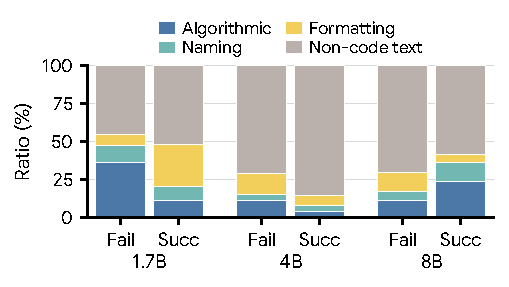
\includegraphics[width=\linewidth]{figures/fig_tstar_semantic_role.pdf}
    \captionsetup{skip=3pt}
    \caption{Semantic-role distribution (\%) of the student token at $\tstar$ across Qwen3 series (SDPO step 0, LiveCodeBench v6). Evaluated by LLM judge (GPT-5.4).}
    \label{fig:tstar-semantic-role}
  \end{minipage}
  \fi
  \begin{minipage}[t]{0.66\textwidth}
    \vspace{0pt}
    \centering
    \begin{subfigure}[t]{0.484848\linewidth}
      \centering
      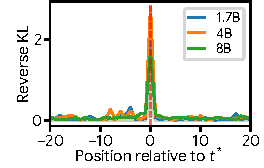
\includegraphics[width=\linewidth,trim=1pt 0 1pt 0,clip]{figures/fig_kl_profile.pdf}
      \caption{Mean per-token KL profile around $\tstar$.}
      \label{fig:kl-profile}
    \end{subfigure}
    \hfill
    \begin{subfigure}[t]{0.484848\linewidth}
      \centering
      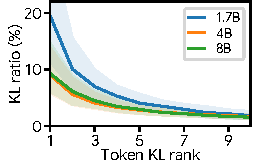
\includegraphics[width=\linewidth,trim=1pt 0 1pt 0,clip]{figures/fig_kl_conc_ratio.pdf}
      \caption{KL concentration ratio by token rank.}
      \label{fig:kl-conc-ratio}
    \end{subfigure}
    \captionsetup{skip=3pt}
    \caption{Concentration of token-level SDPO loss (reverse KL) on failed LiveCodeBench v6 rollouts (Qwen3). \textbf{(a)} Mean per-token KL in a $\pm20$-token window around the peak-divergence position $\tstar$. \textbf{(b)} Fraction of total response KL carried by tokens ranked by KL. The peak token is sharp and consistent across scales, carrying $9$--$20\%$ of total response KL across scales, while the rank-10 contribution is below $1\%$.}
    \label{fig:kl-distribution}
  \end{minipage}
  \hfill
  \begin{minipage}[t]{0.32\textwidth}
    \vspace{0pt}
    \centering
    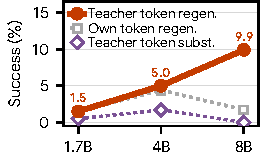
\includegraphics[width=\linewidth,trim=1pt 0 1pt 0,clip]{figures/fig_tstar_continuation_success.pdf}
    \vspace{-4.5pt}
    \captionsetup{skip=0pt}
    \caption{Execution success after intervention at $\tstar$ on failed LiveCodeBench v6 rollouts (Qwen3). \emph{Teacher/own token} force the corresponding action at $\tstar$ and then regenerate the suffix; \emph{substitution} updates only the token at $\tstar$ and preserves the original suffix. }
    \label{fig:tstar-continuation-success}
  \end{minipage}
  \vspace{-0.2cm}
\end{figure*}


\subsection{Peak Divergence Rarely Provides a Local Repair}
\label{sec:analysis-findings}

\paragraph{Peak divergence often occurs outside direct execution decisions.}
On failed rollouts, the semantic role of $t^*$ shifts toward non-code text as model scale increases (Appendix Table~\ref{tab:semantic-role}). Non-code tokens, including comments, docstrings, code fences, and reasoning prose, account for 45.0\% of peak positions at 1.7B and over 70\% at 4B and 8B, while algorithmic tokens decrease from 36.1\% to 11.6\%. Thus, particularly at larger scales, the position of maximal teacher--student disagreement often does not correspond to an explicit algorithmic or control-flow decision. This suggests that peak divergence does not necessarily identify the token directly responsible for execution failure.

\vspace{-0.1cm}\paragraph{Teacher preference alone is rarely a sufficient local repair.}
Directly substituting the teacher-preferred token into the original failed response and rerunning the test suite repairs only $0.0$--$1.7\%$ of failures across model scales (Figure~\ref{fig:tstar-continuation-success}). In contrast, allowing the privileged teacher to generate the suffix from the same intervention point increases success to $7.9\%$ (1.7B), $10.5\%$ (4B), and $13.3\%$ (8B). These results indicate that the teacher-preferred token is rarely sufficient to repair the original trajectory on its own, while changing the continuation after that token can recover a subset of failed responses.

\subsection{A Teacher-Selected Action Can Redirect the Student}
\label{sec:analysis-steering}


\paragraph{A single-token intervention can redirect student generation.}
We force either the teacher's argmax token or the student's original token at $t^*$, then let the student regenerate the suffix in both conditions (Figure~\ref{fig:tstar-continuation-success}). The effect depends strongly on model scale: teacher-token and matched-control success are both $1.5\%$ at 1.7B, differ only slightly at 4B ($5.0\%$ vs.\ $4.4\%$), but separate substantially at 8B ($9.9\%$ vs.\ $1.7\%$). Thus, for Qwen3-8B, the gain cannot be explained by suffix resampling alone: changing only the branch token to the teacher-preferred action leads to substantially more successful student continuations. Of the 24 failed rollouts solved by teacher continuation at 8B, 17 are also solved by the intervened student continuation ($70.8\%$; Appendix Table~\ref{tab:continuation-overlap}).


\subsection{Implications for Trajectory-Level Learning}
\label{sec:analysis-bridge}



The diagnostic motivates disagreement-guided branching as a mechanism for collecting alternative student trajectories. Peak divergence identifies a candidate branch action even when the teacher-preferred token is not sufficient to repair the original response. Forcing this action yields substantially more successful student continuations than the matched resampling control in the larger model (Qwen3-8B). More generally, branching changes the successor prefixes visited by the student, creating contexts that are absent from the original rollout and can therefore receive new privileged-context teacher supervision.
